\documentclass[a4paper, 12pt]{article}

\usepackage{amsmath}
\usepackage{graphicx}
\usepackage{geometry}
\usepackage{color}
\usepackage{hyperref}
\usepackage{listings}
\usepackage[none]{hyphenat}
\usepackage[english]{babel}
\usepackage[backend=bibtex, bibencoding=ascii]{biblatex}
\usepackage{csquotes}
\usepackage{lipsum}
\usepackage{chngcntr}
\renewcommand{\familydefault}{\sfdefault}
\geometry{
	left=1in,
	right=1in,
	top=1in,
	bottom=1in
}

\lstset{
	breaklines=true,
	rulecolor=\color{black}, 
	numbers=left,
	frame = single,
	captionpos=b,
	label=DescriptiveLabel
	}

\lstdefinelanguage{HLSL}
{
	sensitive=true,
	morekeywords=[1]{
	float, float2, float3, float4, float4x4,
	uint, uint2, uint3, uint4,
	RWTexture2D, register, return, if, else
	},
	morecomment=[l]{//},
	morecomment=[s]{/*}{*/},
	morecomment=[l][keywordstyle4]{\#},
}

\counterwithin{figure}{section}

\title{\textbf{Exploration of New Approaches to Depth-Based Render Techniques Utilizing Pixel Synchronization}}

\date{\today}
\author{\textbf{Bryan Pawlowski, Michael Bailey} \\ Computer Graphics \\ \textit{Oregon State University}}

\begin{document}

\begin{titlepage}
\maketitle
\thispagestyle{empty}
\end{titlepage}

\pagenumbering{gobble}
\tableofcontents
\pagebreak

\pagenumbering{arabic}

\section{Introduction and Background} 

Since the advent of computer graphics, engineers have been trying to find new
ways to create graphics hardware solutions intended to yield higher
performance and image quality. However, image quality can mean many things to
many people. Individuals may use grapchics hardware to create vibrant and
abstract experiences, where others may create an experience where the images
being created are as photorealistic as possible. The question that graphics
hardware engineers must ask, is, "What can we make that will help developers
create a higher quality experience?" For some GPU distributors, the solution
comes with a concept called Pixel Synchronization. \\ \\ Before we get into
the gory details of what my project is all about, there are some key concepts
that must be covered. This project utilized a lot of different concepts within
Computer Science outside of the realm of graphics. We first need to cover what
the hardware is and why it is different, then take a general look at the
graphics pipeline, and finally discuss two key topics in parallel programming.
My goal is to make sure my rationale for this project is completely clear.

\subsection{Project Environment Details}
\label{hardware}

At the beginning of this project, we did not have any choices, as far as what
chip/chipset on which to run and test our code. The hardware we used has the
Intel\textsuperscript{\textregistered} Core i7, since this CPU/GPU includes
the Iris\textsuperscript{\texttrademark} Graphics Pro 5200. This project was
developed as a desktop application on Windows 8.1, using the DirectX 11 SDK.
Any and all references to Pixel Synchronization calls are done according to
how they are implemented in the Intel DirectX extensions. Within the
application, all HLSL code was compiled using the HLSL version 5.0, as any
lower version does not support the extensions needed to access Pixel
Synchronization.


\subsection{The Graphics Pipeline}

In modern computer graphics, we describe our objects mathematically as a group
of vertices, then pass them to the graphics card where the vertices are
connected and then drawn to the screen, given constraints we have originally
passed. In the beginning, all we, as graphics programmers could do was tell
the GPU to draw, but then our influence on the graphics was over. Later on,
though, the ability to program stages of the pipeline became possible. With
this programmability of the pipeline, graphics programmers now have the
ability to create and define custom effects for the graphics card to carry out
and process.

\subsubsection{The Vertex Shader}

The Vertex shader is the area of entry for every 3D point. Within the vertex
shader, the GPU generally stores the key information and properties of each
vertex, prior to passing it through to the later stages of the pipeline for
these values to be interpolated. The purpose of this, is that it greatly
reduces the amount of space needed to express the looks and properties of an
object. If we can describe the key pieces of information at a few points on
the object, the idea is that the GPU will be able to make informed assumptions
about the other parts of the model where we have provided no information, thus
filling in/connecting the dots.

\subsubsection{The Pixel/Fragment Shader}

Depending on Direct3D or OpenGL, this stage of the pipeline is either called
the Pixel Shader or the Fragment Shader, respectively. Prior to the Pixel
Shader stage, the 3D object has been transformed, and the object's properties
have been interpolated across its entire surface. After this interpolation
takes place, the GPU then decides where, in screen space, the object is, then
runs the pixel shader to color those specific pixels. Most rendering
techniques do most of their lighting effects and color computations at this
stage of the pipeline to help create a smoother coloring of the model. In a
traditional pipeline, the pixels are evluated in parallel, making rendering a
potentially fast process. The tradeoff, however, is that with increased
rendering speed comes a lack of knowledge of other parts of the object being
evaluated. The more naive the pixel is about its neighbors or its
surroundings, the quicker the computation will finish, and the final image
displayed.

\subsection{Parallel Programming}

Pixel Synchronization and my implementation of these different render
techniques borrow concepts from parallel computing. As vertices are passed
through the pipeline and on to the pixel shader, these parts of the pipeline
are actually happening in parallel for all of the different instances of
vertices and pixels. The problem with doing anything depth-based in realtime
graphics, is that each fragment or potential pixel doesn't really have any
knowledge of any of the neighboring pixels, they do not execute in any
specific order, either. In order to know if one potential pixel is deeper than
another potential pixel, we need a predictable way of determining this. If we
were to naively try to gather this information within the pixel shader, we
would run in to a race condition. We also need a way to share this information
across different instances of the pixel shader.

\subsubsection{Shared Resources}

To determine the depth of a certain spot of a 3D model within the pipeline, we
need some sort of a way for the related potential pixels to communicate with
each other. To do this, we use a feature of Direct3D 11 called Unordered
Access Views. Unordered Access Views (UAVs) are basically a read/write texture
that can only be accessed within the GPU, during the Pixel Shader stage. UAVs
can be used in either a 1 or 2 dimensional array. The size of the UAV is
specified to the graphics device before rendering begins. Within the shader,
the programmer must take care to list the UAVs in the same order as they are
initialized within the CPU side of the application. Once properly initialized,
the UAVs are identified within the shader as RWTexture2D data structures.

\subsubsection{Synchronization and Barriers}

Oftentimes, in parallel programs, we must make sure our threads (or in the
case of this project, pixels) are synchronized and executed in some sort of
order. If we know that our programs are executed in some predictable order, it
is easier for us to write more advanced algorithms or have guaranteed
knowledge of what data lies at each checkpoint. If barriers did not exist, we
come across \textbf{race conditions}. When an algorithm is written where race
conditions exist, it is difficult, or impossible to predict the output of the
algorithm, itself.

\subsection{Pixel Synchronization}

\subsubsection{What is Pixel Synchronization?}

With Pixel Synchronization, the pipeline is now capable of creating a barrier
during the pixel shader stage per pixel, where multiple instances of the pixel
being rendered will happen in-order, based on the primitive number. Parallel
programming concepts such as barriers and synchronization have not before been
possible within the real-time pipeline. To have this emerging hardware
capability gives programmers the opportunity to approach existing render
techniques from a new angle, potentially yielding higher performance and more
spectacular images.

\subsubsection{How Pixel Synchronization Works in Code}

\nohyphens{On the programmer side, there is not much coding overhead as far as
initializing, then calling Pixel Synchronization. On the application side, the
programmer must first check the hardware to make sure that the hardware is
capable of Pixel Synchronization. This is the only thing to be done on the
application side. Within the pixel shader, we have to first enable Pixel
Synchronization with a call to \textbf{IntelExt\_Init()}. Then, once we reach
the part of our code that must be syncrhonized, we must call the pixel
ordering function by calling \textbf{IntelExt\_BeginPixelShaderOrdering()}
(\textbf{NOTE:} These function calls are hardware specific. Please see section
\ref{hardware} on page \pageref{hardware} for details about the hardware used
for this project). An important point to keep in mind is that this specific
implementation of Pixel Synchronization lasts until the end of the Pixel
Shader code. What this means, is that it is recommended that all code over
which syncronization must occur should come as close to the end as possible.
Listing \ref{code:PSExample} (below) shows how a bare bones Pixel Shader using
Pixel Synchronization might look.}


\begin{figure}[h]
\begin{lstlisting}[language=HLSL]
float4 PSExample(/*parameters...*/) : SV_TARGET
{

	//Variable Definitions

	IntelExt_Init();
	
	//all non synchronization-specific code;

	IntelExt_BeginPixelShaderOrdering();

	//all synchronization-specific code goes here
	//critical section must happen at the end.

	return finalColor;
}

\end{lstlisting}
\caption{How Pixel Synchronization Pixel Shader Code Might Look}
\label{code:PSExample}
\end{figure}

\pagebreak


\section{Simple Subsurface Scattering}

\subsection{What is Subsurface Scattering?}

Subsurface Scattering is a phenomenon which occurs when photons hit some sort
of translucent material, such as skin, fat, milk, plant leaves, etc. The
photons enter that material, scatter, then exit out of a different point. This
phenomenon is constantly and naturally occuring in the real world, but it is a
rather tough lighting effect or phenomenon to calculate in realtime graphics,
since knowledge of the object, and sometimes its surrounding environment, is
required to produce an image with accurate subsurface scattering effects. Even
so, many approximate implementations have been developed to mimic this natural
phenomenon as convincingly as possible, all while retaining
performance/framerate. \\ \\ All of the techniques out there attempt to find a
fast way to build knowledge of the 3D object (what is its depth at a certain
point, and where is it with respect to the light). The techniques that exist
are either quite general, or are very complex, coding wise (further detail to
come below). Pixel Synchronization offers a new approach to the subsurface
scattering problem that is both straightforward and does not sacrifice
performance.

\subsection{Previous Implementations}

As stated above, there exist approaches to approximating the subsurface
scattering effect in realtime graphics. The two approaches detailed below have
trade-offs, when it comes to generality or coding complexity. However, both
methods are quite effective within the correct scope. With the Pixel
Synchronization approach detailed in section 
\ref{section:PSDepthMap} (pg.\pageref{section:PSDepthMap}), we hope to improve
upon these two methods by creating a more detailed and accurate approach,
while keeping the code intuitive.

\subsubsection{Wrapping Approximation}
\label{section:wrapping}
This simple approach to a subsurface scattering approximation takes the
calculation of the diffuse component of your standard Phong lighting equation,
and basically "wraps" the diffuse around the object further than the standart
diffuse calculation. For instance, is illustrated in the equation in Figure
\ref{equation:diffuse} (where $L$ is the light vector and $N$ is the normal
vector).

\begin{figure}[h]
\[diffuse = max(0, L \bullet N)\]
\caption{Standard diffuse calculation in smooth shading}
\label{equation:diffuse}
\end{figure}

\noindent However, when we apply the wrapping approximation, the equation for
the diffuse component is slightly changed. In Figure \ref{equation:wrap}, the
programmer specifies a wrap value, or makes the value interactive to show the
difference in realtime, then the value is applied to the existing equation as
follows:

\begin{figure}[h]
\[diffuse = max(0,((L\bullet N) + wrap) \div (1 + wrap))\]
\caption{Diffuse Calculation in smooth shading with wrap value added}
\label{equation:wrap}
\end{figure}


\noindent As can be seen by observing the above equations, the addition of the
wrapping value in equation complicates it only slightly, but the effect of
adding the is very apparent. The advantage to this approach is that it
requires only a slight modification of Phong illumination. Within shader code,
a graphics programmer could insert a hook in their shader code to show the
difference between Phong Illumination with and without diffuse wrapping. For
an idea on how this is implemented, refer to the code listing in figure
\ref{code:WrapExample}.

\begin{figure}[h]
\begin{lstlisting}[breaklines, language=HLSL]
float calc = dot(Normal, Light) + wrap) / 1 + wrap);
if(mode & DIFFUSE_WRAP) d = max(calc, 0);
else d = max(dot(Normal, Light), 0);
\end{lstlisting}

\caption{HLSL hook to determine whether or not to wrap the normal}
\label{code:WrapExample}
\end{figure}

\noindent In line 2, a bitwise 'and' operator is used to check if wrapping has
been selected because all display mode settings are passed into the graphics
program as a single unsigned integer (in OpenGL, this would be the same as
passing in a single uniform variable to evaluate all user true-false settings.
This saves time and space when passing these types of variables to the GPU). A
more detailed discussion about this and why this approach for uniform
variables is used can be found in section \ref{subsection:Implementation} on
page \pageref{subsection:Implementation}.

\subsubsection{Depth Mapping} 
\label{section:DepthMap}

Given the nature of what Subsurface Scattering is, it is imperative to know
the thickness of the object in question, such that the programmer can make a
decision on how much light escapes the obejct at a different point. For this
reason, a technique was developed called depth mapping. In the first pass, the
scene is rendered from the light's position, toward the object, where we store
the distance from the light to that location on the object. Another pass is
made to measure where the ray has entered and exited, by mapping the depths to
the object's texture space. Finally, in the render pass, we render the object
from the camera's point of view, and for each point on the object being
rendered, we find the point of entry and the point of exit for the specific
ray pertaining to the current fragment of the object, then calculated the
distance between the two. After this distance has been calculated, the new
calculation of the diffuse light can be applied. For a visual representation
of the render pass of the approach, see figure \ref{pic:DepthMap} on page
\pageref{pic:DepthMap}. \\ \\ The effect from this approach causes more of a
subsurface scattering type of "lifelike glow" than the method detailed in
Section \ref{section:wrapping}. However, when this method is implemented, it
requires three passes to render the image with correct depth information.
Further, there is no intuitive way to project the the depth information with
respect to the light to the object. To recap, here are the three render passes
that take place.



\begin{figure}[h]

\begin{description}

\item[First Pass] \hfill \\ Render the object from the perspective of the
light and record the distances from the light.

\item[Second Pass] \hfill \\ Calculate the distances between the entry and
exit points of the light rays. These will be mapped, in texture space, to the
object.

\item[Third Pass] \hfill \\ Use the depth calculations to scale the backfacing
(with respect to the light) diffuse component of the object.

\end{description}
\caption{Description of the depth mapping approach to subsurface scattering}
\label{figure:depthDesc}
\end{figure}

\begin{figure}[h!]
	\centering
	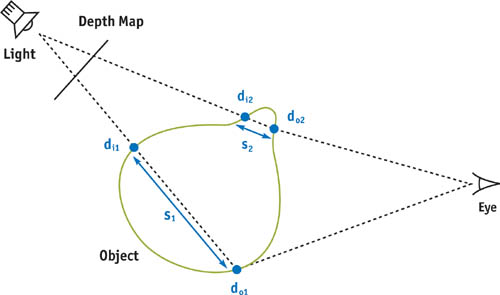
\includegraphics[width=1.0\textwidth]{depthMap.jpg}
	\caption{Diagram to visualize how the depth map is used to calculate the distance a light ray has traveled within a 3D object}
	\label{pic:DepthMap}
\end{figure}



\subsection{Pixel Synchronization Accelerated Depth Mapping}
\label{section:PSDepthMap}

The approach described in section \ref{section:DepthMap} is the groundwork for
the new Pixel Synchronization accelerated approach. The concept remains
relatively the same, however, we are able to use a psuedo raytrace to guage
the distance between two points in the same ray with increased ease. This more
straighforward approach to depth mapping takes less time to code and yields no
loss of performance.

\subsubsection{In-Depth Description of Implementation}

As stated above, the approach to this technique remains generally the same,
but with a few differences. For clarity's sake, refer to the description in
\ref{figure:depthDesc} as a reference to what the changes in the pixel shader
based approach would be, in comparison to the description below.

\begin{figure}[h!]

\begin{description} 

\item[First Pass] \hfill \\ 

This pass remains relatively the same. We take this pass to map which pixel
from the perspective of the light. However, we map the object to the screen
with respect to its texture coordinates. This way, we guarantee that all of
the object is being seen and processed by the GPU. For a better idea of what
this means, see the listing \ref{code:VShaderPSDepth} on page
\pageref{code:VShaderPSDepth}. More specifically, see lines 6 through 8. Here,
we take the text coordinates, then convert them into a space spanning from -1
to 1 in the x and y axes. Then, when these positions are passed from the
vertex to the pixel shader, they are converted to screen space. \\ \\ After
this screen space conversion, we calculate and store the distance of each part
of the model from the light source. Following this, we then map which rays
intersect which parts of the model in 3D space. This is why we also store and
keep track of the 3D position of the model, as seen on line 11 in listing
\ref{code:VShaderPSDepth}. We map these ray values (which coincide with the
pixels) to another texture, which we will use in the next pass as a "mask."
For an idea of these mappings, refer to \ref{code:PixelShaderPSDepth} on page
\pageref{code:PixelShaderPSDepth}. We use Unordered Access Views to accomplish
these mappings (\ref{section:UAVs}, page \pageref{section:UAVs}).

\item[Second Pass] \hfill \\  

This pass is from the perspective of the light, but this time, we project the
correct object into space, rather than its texture coordinates. The only
difference here, is that $output.svposition$ gets $mul(final, position)$
rather than the calculated screen space coordinates as it does in line 9 of
figure \ref{code:VShaderPSDepth}. However, within the Pixel Shader this time,
we create our shallow mask. This is basically a UAV-created depth buffer to
keep the shallowest positions with respect to the light. To see how this is
implemented within the shader, please see listing \ref{code:POShader} on page
\pageref{code:POShader}. With the aid of Pixel Synchronization, we can determine which parts of the object are closest to (facing) the light.

\item[Third Pass] \hfill \\ 

The final render pass remains the same as what we had in the approach on page
\pageref{section:DepthMap}. We take the current depth, with respect to the
light, then compare it to the corresponding member of the shallow mask. For a
coding example, turn to page \pageref{code:PSDepthRender} and see figure
\ref{code:PSDepthRender}. The code block from lines 6 to 25 show how to both
get the ray and the current light-based depth of the object, compare them, and
then re evaluate the diffuse component, originally calculated above this
section Other parts of the shader were edited out for the sake of readability
and clarity. There will be a complete discussion on the code within
$PSHader2()$ later on in this paper. We can get away with using array
notation, since UAVs support access via array notation, and not with a call to
$sample()$.

\end{description}
%\caption{Description of the depth mapping approach to subsurface scattering}
\label{figure:PSDesc}
\end{figure}
\begin{figure}[h!]
\begin{lstlisting}[breaklines=true, language=HLSL]
VOut VShader(...)
{
	VOut output;

	float2 movedCoords = texCoord * 2;
		movedCoords.x -= 1;
		movedCoords.y -= 1;
	float4 svPos = float4(movedCoords, 0.0, 1.0);
	output.svposition = svPos;
	output.position = mul(final, position);

	// set the ambient light
	output.color = ambientcol;

	
	float4 norm1 = normalize(mul(rotation, normal));
	float diffusebrightness = saturate(dot(norm1,lightvec));
	float4 norm = normalize(mul(final, normal));

	//output.color += lightcol * diffusebrightness;

	output.UVs.x = texCoord.x * SCREEN_WIDTH;
	output.UVs.y = texCoord.y * SCREEN_HEIGHT;

	output.normal = norm;

	output.camera = mul(final, lightPos);

	output.mode = mode;


	return output;
}
\end{lstlisting}
\caption{Vertex Shader for first Pass of Depth Map accelerated by Pixel 
Synchronization}
\label{code:VShaderPSDepth}
\end{figure}

\begin{figure}[h!]

\begin{lstlisting}[breaklines=true, language=HLSL]
float4 PShader(...) : SV_TARGET 
{
	float2 svPos = position.xy;
	float mdepth = distance(position, camera);
	uint2 uv = UVs;

	svPos.y = 0 - svPos.y;
	svPos += 1;
	svPos = svPos / 2;

	float2 newPos;

	newPos.x = svPos.x * SCREEN_WIDTH;
	newPos.y = svPos.y * SCREEN_HEIGHT;

	fromLightX[uv] = newPos.x;
	fromLightY[uv] = newPos.y;
	uvDepth[uv] = mdepth;

	return color;
}
\end{lstlisting}
\caption{Pixel Shader from first pass of Pixel Synchronization-Accelerated 
depth mapping.}
\label{code:PixelShaderPSDepth}
\end{figure}

\begin{figure}[h!]
\begin{lstlisting}[breaklines=true, language=HLSL]
float4 POShader(...) : SV_TARGET
{
	uint2 pixelAddr = svposition.xy;

	float pos = distance(position, camera);

	IntelExt_Init();
	IntelExt_BeginPixelShaderOrdering();

	if (pos < Shallow[pixelAddr])
	{
		Shallow[pixelAddr] = pos;
	}

	return color;
	
}

\end{lstlisting}
\caption{Pixel Ordering step of the alternate approach to depth mapping}
\label{code:POShader}
\end{figure}

\begin{figure}[h]
\begin{lstlisting}[breaklines=true,language=HLSL]
float4 PShader2(...)
{

	/*...*/

	if (!(mode & PHONG_RENDER))
	{
	  uint2 lightCoords;

	  lightCoords.x = fromLightX[uv];
	  lightCoords.y = fromLightY[uv];

	  float mdepth = uvDepth[uv];

	  float shallow = Shallow[lightCoords];
	  if ((mode & PIXSYNC_OFF) && 
	      (uvDepth[uv] > Shallow[lightCoords])){
		  
		  float4 lColor = lightcol;
		  lColor -= 
		    (uvDepth[uv] - Shallow[lightCoords]) * 3;
			
		  diffuse += lColor;
	  }
	}

	/*...*/
}
\end{lstlisting}

\caption{Render Pass from perspective of camera}
\label{code:PSDepthRender}
\end{figure}

\pagebreak

\section{Refraction}

Refraction is a visual phenomenon that occurs when a translucent object, such
as a glass figurine, bends light in such a way that it distorts the image
beyond it. This is how real-life lenses accomplish vision correction, or the
image of an object gets distorted when it is submerged in water. As humans, we
rely on refraction a great deal, so we are very, very used to seeing this
effect on a day-to-day basis. There are many ways to accomplish the
approximate effect of refraction on the GPU. The first approach, detailed in
section \ref{section:SimpleRefract}, is a simple refraction algorithm, that
takes into account only the front face of the object to compute the color of
the object at that point.

\pagebreak

\subsection{"Fake" Convex Object Refraction}
\label{section:SimpleRefract}

The most used approach to refraction is to just bounce the viewing "ray" once
on the front surface of the object, then samples the cubemap to return a
color. In code, this effect requires just a Vertex and Pixel Shader.

\subsubsection{Vertex Shader}

All of the heavy-lifting for refraction is done within the Vertex Shader
(\ref{code:VSSimpleRefract}). Given the proper transform and rotation
matrices, the refract vector is computed within the Vertex shader.
Essentially, the distance between

\begin{figure}[h]
\begin{lstlisting}[breaklines=true,language=HLSL]
VOUT VShader(...)
{

	VOUT output;

	output.svPos = mul(WVP, pos);
	output.Pos = mul(WVP, pos);
	float4 norm = mul(Rotation, normal);


	float diffusebrightness = 
			saturate(dot(norm, LightVector));

	float3 ECPosition = mul(World, pos).xyz;
	float3 eyeDir = float3(0.0f, 0.0f, 0.0f) - ECPosition;
	
	output.Color = AmbientColor;

	output.Color += LightColor * diffusebrightness;
	output.Normal = norm;
	output.texCoord = texCoord;

	float3 reflectVector = refract(norm, eyeDir, -.90);

		output.vRef = reflectVector;


	return output;
}
\end{lstlisting}

\caption{Vertex shader for simple refraction}
\label{code:VSSimpleRefract}
\end{figure}

\begin{figure}[h]
\begin{lstlisting}[breaklines=true,language=HLSL]
float4 PShader( VOUT input ) : SV_TARGET
{	
	float3 bounceVec = input.vRef.xyz;
	
	float4 newColor = 
	 SkyMap.Sample(ObjSamplerState, normalize(bounceVec));
	
	return newColor;
}
\end{lstlisting}

\caption{Pixel shader for simple refraction}
\label{code:PSSimpleRefract}
\end{figure}

\subsection{Better Convex Refraction With Pixel Synchronization}

The idea behind this approach is to create a volumetric representation of the
scene which stores the object's surface normals, with respect to the eye. For
the render step, we could step through this voxelization at the entrypoint,
then trace the first refracted ray to the exit point, refract again, then
return this double-refracted color to give a more accurate coloring of the
pixel.

\subsubsection{Shader-Based Description of Implementation}

To get our volumetric representation, I attempted (see section
\ref{subsection:Implementation} for more details) to utilize the shader to
take care of that for me. Using Pixel Ordering, I tried to create a voxel-
based representation of the entire scene. I tried to use two 3D textures to
accomplish this. One 3D texture would have $unsigned int$ representations of
every voxel element saying whether it was inside, outside, or on the face of
the object within the scene:

\begin{description}
\item[0:] outside of the object
\item[1:] on the object's face
\item[2:] inside of the object
\end{description}

\noindent The suface normals are stored in another 3-D texture. We would first
mark all of the spaces according to the above description. The surface normal
texture is populated at the beginning of populating this unsigned integer
texture. How this texture is populated can be better described by the code
within figure \ref{code:3DTexPop}. On line 8, we begin our loop to populate
the 3D texture. As can be seen, pixel ordering has been invoked within this
shader. So, what we do is step through our $unsigned int$ Texture3D at every
pixel address, in order. this way, we are able to indicate which parts of the
scene are inside or outside of the model. We keep another 3D texture to keep
track of the surface normals. The idea behind this, was once we hit an index
in the $unsigned int$ Texture3D of value 1, we could then use that index where
the 1 value is to refract the ray further, since that is where the surface
normal at that point is stored in the other Texture3D. Using these textures in
tandem serves as a good way to trace through a solid object to find the
accurate refraction. However, I didn't get as far as a tracing stage to my
algorithm, as there are fundamental aspects of this algorithm that GPU
compilers do not allow to happen, due to memory access restrictions. This will
be covered in more detail in section \ref{subsection:Implementation}, where
the implementations will be discussed. However, the source code for this
attempted demo will still be included in my final source code.

\begin{figure}[h]
\begin{lstlisting}[breaklines=true,language=HLSL]
float4 PShader(...)
{

	IntelExt_Init();
	IntelExt_BeginPixelShaderOrdering();

	/*...*/

	uint3 tempi = voxPos;

	[loop]
	for (i = voxPos.z + 1; i < 512; i++)
	{
		tempi.z = i;
		unsigned int cond = VoxMask[tempi];
		if (cond == 0)
		{
			VoxMask[tempi] = 2;
			continue;
		}
		else if(cond == 2)
		{
			VoxMask[tempi] = 0;
			continute;
		}
		break;
	}
	/*...*/
}
\end{lstlisting}
\caption{Populating the \textit{unsigned int} 3D texture.}
\label{code:3DTexPop}
\end{figure}

\section{Findings and Observations}

There are a lot of quirks and behaviors that have been logged throughout the
entirety of this project. Firstly, I'd like to touch on the performance
metrics of my project, and compare how it stacks up with existing algorithms,
performance-wise, and also give a side-by-side comparison of the output images
to show whether or not utilizing pixel synchronization to simulate a depth-
based technique, such as a Subsurface Scattering approximation is worth it.

Following performance metrics, I will write about my observations of how the
hardware, itself works, UAVs, and how they work, and then small coding
oddities I found along my way toward my finishing my project. Included will be
photos demonstrating behavior, along with explanations and recommendations on
how to deal with these issues. The following sections are key to knowing how
this hardware works, to extend to projects that use explore this same type of
hardware (nVidia's Pixel Interlock technology, for example). Reading through
this section should save time on the setup and boilerplate side of things.

\subsection{Performance Metrics}
\label{section:findings}
\subsubsection{Raw Performance Check of Pixel Synchronization}

\lipsum[22-23]

\subsubsection{Subsurface Scattering}

\lipsum[24-38]

\subsubsection{Refraction}

\lipsum[39-53]

\subsection{Observations}

\subsubsection{Unordered Access Views}
\label{section:UAVs}

\lipsum[54-59]

\subsubsection{Pixel Synchronization Behavior}

\lipsum[60-74]

\subsubsection{Coding Quirks}

\lipsum[75-99]


\subsubsection{Suggestions and Advice When Using Pixel Synchronization}

\lipsum[100-114]

\pagebreak

\section{Conclusion and Recommended Future Work}

\lipsum[115-119]

\subsection{Implementation Discussion}
\label{subsection:Implementation}

\lipsum[120-150]

\subsection{What Do These Findings Mean?}

\lipsum[1-19]

\subsection{Where Do We Go From Here?}

\lipsum[20-75]

\end{document}